\documentclass{beamer}
\usepackage[T1]{fontenc}
\usepackage{microtype}

\input{preamble.tex}

\title{Computer Language Processing}
\subtitle{Lab 1}
\author{Noé De Santo}
\date{Fall 2021}

\begin{document}
    \frame{\titlepage}

    \section{The big picture}

    \begin{frame}{The pipeline}
        You will implement a full compiler/interpreter for 
        a programming language called Amy.

        \centering
        \dotgraph{pipeline}
    \end{frame}

    \begin{frame}{The labs}
        \begin{itemize}
            \item Lab01 -- Interpreter;
            \item Lab02 -- Lexer;
            \item Lab03 -- Parser;
            \item Lab04 -- Type Checker;
            \item Lab05 -- Codegen (Code Generator);
            \item Lab06 -- Compiler extension.
        \end{itemize}
    \end{frame}


    \section{The interpreter}

    \begin{frame}[fragile]{Interpreting source code}
        From:
        \code{Hello.scala}

        To:
        \terminal{Hello.out}

    \pause
        \vspace{2em}
        But that would be a bit difficult to do at once ...
    \end{frame}

    \section{The interpreter \emph{phase}}

    \begin{frame}{Lab01}
        \dotgraph{pipeline_hg}

        We "only" have to interpret the result of the front end.

        The front end (which you will implement in labs 2,3\&4) 
        produces a data structure called an \emph{Abstract Syntax Tree (AST)}.
    \end{frame}


    \begin{frame}[fragile]{Interpreting an AST}
        From:\\
        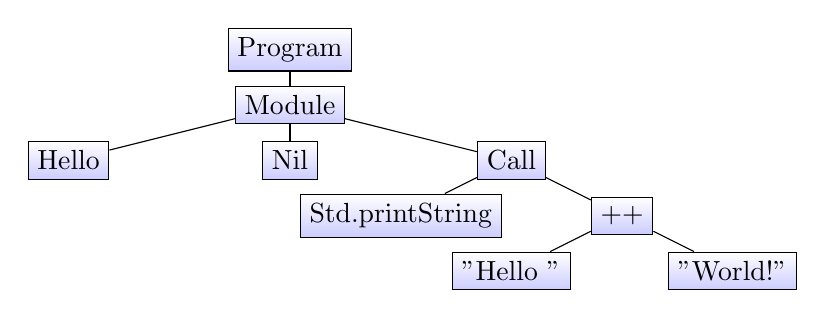
\begin{tikzpicture}[sibling distance=8em, level distance=2em,
            every node/.style = {shape=rectangle,
                draw, align=center,
                top color=white, bottom color=blue!20}]]

            \node {Program}
                child { node {Module} 
                    child { node {Hello} }
                    child { node {Nil} }
                    child { node {Call}
                        child { node {Std.printString} }
                        child { node {++}
                            child { node {"Hello "} }
                            child { node {"World!"} }
                        } 
                    }
                }
            ;

        \end{tikzpicture}

        
        To:
        \terminal{Hello.out}

        An approximate definition of the AST is available on gitlab\footnote{\url{\asturl}}.
    \end{frame}

    \section{Doing the lab}

    \begin{frame}{The \mintinline{scala}{interpret} function}
        You have to complete (in {\footnotesize\texttt{src/amyc/interpreter/Interpreter.scala}})
        \code[fontsize=\scriptsize]{Interpret.scala}
        \begin{itemize}
            \item<2-> \mintinline{scala}{expr} is the AST to interpret, e.g.
                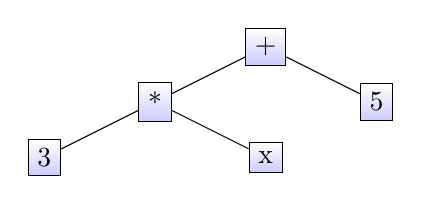
\begin{tikzpicture}[sibling distance=8em, level distance=2em,
                    every node/.style = {shape=rectangle,
                        draw, align=center,
                        top color=white, bottom color=blue!20}]]
        
                    \node {+}
                        child { node {*}
                            child { node {3} }
                            child { node {x} }
                        } 
                        child { node {5} }
                    ;
        
                \end{tikzpicture}

            \item<3-> \mintinline{scala}{locals} maps variable identifiers into their values, e.g. 
            \code{Locals.scala}
        \end{itemize}
    \end{frame}

    \begin{frame}[fragile]{Workflow}
        \begin{itemize}
            \item<1-> 
            Locate the {\footnotesize\texttt{???}}s:
            \code{Times_missing.scala}

            \item<2-> Refer to the amy specification\only<2->{\footnote{\url{\specsurl}}} (section 3.5)
            for the expected behavior of the expression:

            \begin{quote}
                « \gtns{+}, \gtns{-}, \gtns{*}, \gtns{/} and \gtns{\%} 
                have type \typeII{\Int}{\Int}{\Int},
                and are the usual integer operators. »
            \end{quote}

            \item<3-> Implement the required semantic:
            \code{Times.scala}

        \end{itemize}

    \end{frame}

    \begin{frame}[fragile]{The front end is nice}
        The front end will reject non-sensical 
        programs\only<2->{\footnote{Useless fact: \mintinline{js}{"Amy <3" || 5} is valid in javascript; it evaluates to \mintinline{js}{"Amy <3"}}}

        \pause
        \code{Bogus.scala}

        \pause

        \terminal[fontsize=\fontsize{7}{8}]{Bogus.out}


        So you can assume that the AST always represents a valid program.
    \end{frame}

    \begin{frame}{We provide some tests...}
        \codeblock{tests/EmptyObject.scala}{EmptyObject.scala}

        \vspace{1em}

        \codeblock{tests/MinimalError.scala}{MinimalError.scala}

        \pause
        ...but you should write your own.

    \end{frame}

    \begin{frame}{A word from your head-TA}
        \begin{quote}
            «If I were to take something from this course, it would be learning to write good tests»
        \end{quote}
        {\begin{flushright} \footnotesize Rodrigo \end{flushright}}
    \end{frame}


    \begin{frame}{Tips and tricks}
        \begin{itemize}
            \item Read The Fine Manual: 
            the specification\footnote{\url{\specsurl}} contains every information you need:
            \begin{itemize}
                \item Section 1 explains most features of Amy;
                \item Section 3 contains crucial details for this assignment;
                \item Reading section 2 might also help you understand some intricacies of Amy;
            \end{itemize}

            \item Even though the file is not included in the skeleton, 
            {\footnotesize\texttt{SymbolicTreeModule.scala}}\footnote{\url{\asturl}} 
            is useful to know what the fields
            of the different nodes of the AST are;

            \item The handout and the comments contain some additional hints on how to implement
            some of the most difficult parts;

            \item You can run examples/tests even with an incomplete interpreter.
        \end{itemize}

    \end{frame}

    \begin{frame}[plain]{}
        \centering \Large \bfseries
        Good Luck !
    \end{frame}

    \section{Q\&A}

    \begin{frame}{Q\&A}
        \begin{qaalist}
            \qaa{Should we merge our code in main/master when done ?}{
                No, but you will usually have to merge 
                your code into the new labs, e.g. merge lab02 into lab03.
            }
        \end{qaalist}
    \end{frame}

\end{document}